\documentclass[12pt]{article}
\usepackage[utf8]{inputenc}
\usepackage{authblk}
\usepackage{graphicx} % Lib de importar e tratar imagem
\usepackage[english,brazil]{babel} % Manter dois idiomas
\usepackage{fancyhdr} % Configuração das paginas
\usepackage{float}
\usepackage{xcolor}
\usepackage{titlesec}
\usepackage{background} % Componente de Watermark
\usepackage{hyperref}

% Definir as características do hyperlink
\hypersetup{
    colorlinks=true,
    linkcolor=blue,
    filecolor=magenta,      
    urlcolor=cyan,
    pdftitle={Overleaf Example},
    pdfpagemode=FullScreen,
}

%Função para diminuir tamanho da fonte
\newcommand{\changefont}{%
    \fontsize{9}{12}\selectfont
}

%Document Layout Config
\pagestyle{fancy}
\setlength\headheight{26pt}
\setlength\parindent{0pt}
\fancyhf{}
% Header  Config
\fancyhead[RO]{Ataque Terrapin}
% Footer  Config
\renewcommand{\footrulewidth}{0.4pt} % Inserir linha no final da pagina "pre-footer"

%Document Specification
\title{Ataque Terrapin}
\author{Caio Abreu Ferreira}
\affil{Análise técnica do Ataque Terrapin}
\date{\selectlanguage{brazil}\today}
\graphicspath{ {img/} }

%Capa
\begin{document}
\backgroundsetup{contents={}} %Remover a palavra Draft da página
\NoBgThispage % Ignorar background na capa
\maketitle
\pagenumbering{gobble} % Não contar como página a capa
\pagebreak

%Resumo Executivo
\section*{\centering{Resumo Executivo}}
\vspace*{\fill}
\large{	O ataque cibernético denominado Terrapin representa uma ameaça significativa, visando o protocolo SSH amplamente empregado por administradores de sistemas para acesso remoto. A exposição desse protocolo ressalta a necessidade crítica de medidas preventivas e de mitigação. Dada a larga utilização do protocolo SSH na infraestrutura de TI, a proteção contra o Terrapin torna-se necessário. A consciência e a ação proativa diante dessa ameaça são essenciais para preservar a estabilidade e a segurança.}
\vspace*{\fill}
\fancyfoot[CO]{\changefont Este documento está licenciado sobre a licença Creative Commons BY-NC-SA}
\pagebreak

%Sumario
\tableofcontents
\pagebreak

%Texto rodapé
\fancyfoot[CO]{\thepage\\\changefont Este documento está licenciado sobre a licença Creative Commons BY-NC-SA}
\pagenumbering{arabic}
\section{Introdução}

O Ataque Terrapin representa uma ameaça significativa ao protocolo criptográfico SSH. O protocolo SSH é amplamente empregado por administradores de sistemas para acessar servidores remotamente. Este ataque compromete a segurança do SSH ao realizar um downgrade por meio de uma interceptação man-in-the-middle. O presente texto constitui uma análise técnica detalhada desse ataque.

%Page
\section{Protocolo SSH}

\subsection{O que é}
Desenvolvido com o propósito de substituir protocolos não criptografados, como Telnet e RSH, e protocolos de transferência de arquivos desprotegidos, como FTP e RCP, o SSH estabelece conexões seguras e criptografadas entre dois dispositivos. Os administradores empregam predominantemente o protocolo SSH para realizar logins remotos, acessar máquinas em suas redes, efetuar transferências de arquivos, executar comandos e administrar aplicações.

\subsection{Como funciona}
O funcionamento do protocolo segue o modelo cliente-servidor, em que a conexão é iniciada pelo cliente SSH, estabelecendo conexão com o servidor SSH. O cliente SSH inicializa o processo de estabelecimento da conexão, utilizando criptografia do tipo chave pública-privada para autenticar o servidor SSH. Após a fase de configuração, o protocolo SSH utiliza criptografia do tipo simétrica e algoritmos de hashing para assegurar a privacidade e integridade dos dados trocados entre cliente e servidor.\\

A Figura \ref{fig:protocolo_ssh} apresenta um fluxo de configuração simplificado de uma conexão shell segura.

\begin{figure}[H]
	\centering
	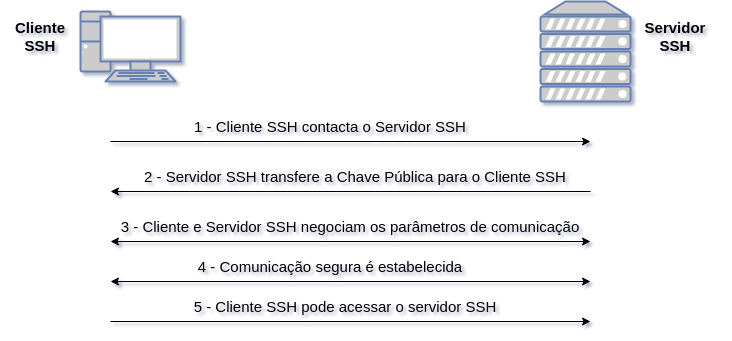
\includegraphics[scale=0.63]{protocolo_ssh.png}
	\caption{Descrição do funcionamento do protocolo SSH}
	\label{fig:protocolo_ssh}
\end{figure}

\begin{enumerate}
	\item Por meio de um software gráfico ou utilizando a linha de comando, o Cliente SSH estabelece a comunicação inicial com o Servidor SSH por meio do protocolo TCP;
	\item O servidor SSH transmite a Chave Pública utilizando o algoritmo de criptografia RSA assimétrico;
	\item O Servidor SSH e o Cliente SSH trocam informações relativos ao protocolo de criptografia e outras informações pertinentes durante a comunicação;
	\item Após a confirmação e estabelecimento da comunicação entre as partes envolvidas, ambas utilizam o que é conhecido como Chave de Algoritmo de Troca Diffie-Hellman para gerar uma chave simétrica. Esse algoritmo possibilita que tanto o Cliente quanto o Servidor compartilhem uma chave criptografada do tipo simétrica, algoritmo de criptografia AES 256, a qual será empregada para conduzir a sessão de comunicação;
	\item Este é o último estágio antes de o usuário obter suas credenciais de acesso ao servidor de forma autenticada. Nesse sentido, os usuários de SSH utilizam uma senha como meio de autenticação.
  \end{enumerate}
\pagebreak

%Page
\section{Terrapin}

\subsection{Descrição}

O Terrapin é um tipo de ataque direcionado ao protocolo SSH que compromete a integridade do canal seguro. Especificamente, esse ataque manipula os números de sequência durante o processo de handshake, permitindo que um invasor elimine mensagens enviadas pelo cliente ou servidor no início do canal seguro sem detecção.\\

Este tipo de ataque pode ser executado na prática, resultando na diminuição da segurança da conexão ao truncar a mensagem de negociação de extensão da transcrição. Isso pode levar à adoção de algoritmos de autenticação menos seguros pelo cliente e à desativação de contramedidas específicas contra ataques de temporização de pressionamento de tecla no OpenSSH 9.5.\\

O Terrapin também pode ser explorado para aproveitar falhas na implementação do protocolo SSH, possibilitando ataques de phishing e concedendo ao invasor recursos de Man-in-the-Middle (MitM) dentro da sessão criptografada.\\

Para realizar o ataque Terrapin, é necessário ter recursos MitM na camada de rede para interceptar e modificar o tráfego da conexão. Além disso, a conexão deve ser protegida pelos algoritmos de criptografia \textbf{ChaCha20-Poly1305} ou \textbf{CBC com Encrypt-then-MAC}" para permitir o ataque.\\

\subsection{Mitigação}

Para mitigar o ataque Terrapin em um servidor ou cliente do tipo OpenSSH, é imperativo que o administrador de sistemas modifique os arquivos de configuração do OpenSSH, o arquivo \textbf{ssh\underline{\hspace{.1in}}config} para o cliente e o arquivo \textbf{sshd\underline{\hspace{.1in}}config} para o servidor e altere os arquivos para que fiquem igual as linhas abaixo.

\begin{itemize}
    \item \small \textbf{Ciphers aes256-gcm@openssh.com,aes128-gcm@openssh.com,aes256-ctr,aes192-ctr,aes128-ctr}
    \item \small \textbf{MACs hmac-sha2-512,hmac-sha2-256,umac-128@openssh.com}
\end{itemize}

O comando acima irá remover o algoritmo de criptografia \textbf{ChaCha20-Poly1305} e o algoritmo de MAC \textbf{-etm@openssh.com} do processo de autenticação.\\

A Figura \ref{fig:terrapin_depois} exemplifica uma tentativa de conexão utilizando o algoritmo de criptografia \textbf{ChaCha20-Poly1305} e a recusa da conexão pois o algoritmo de criptografia não é mais suportado pelo servidor SSH.

\begin{figure}[H]
	\centering
	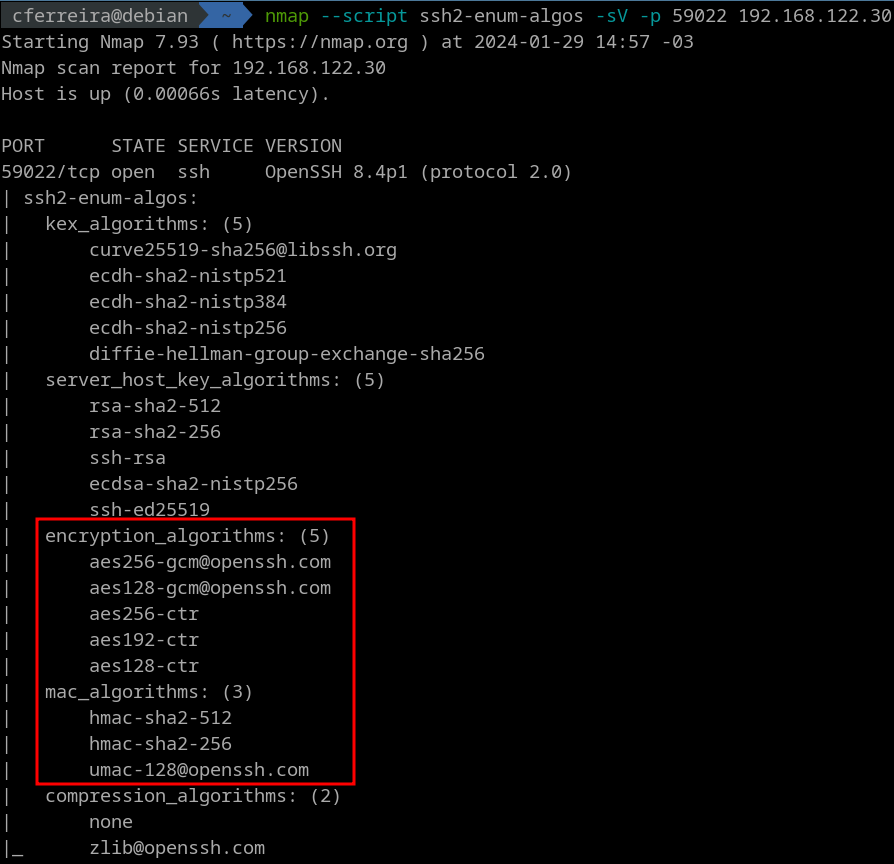
\includegraphics[scale=0.50]{terrapin_depois.png}
	\caption{Algoritmos utilizados pelo OpenSSH}
	\label{fig:terrapin_depois}
\end{figure}

Nas demais implementações do protocolo SSH, recomenda-se avaliar a eventual necessidade de modificar o arquivo de configuração ou realizar a atualização do software correspondente.

\pagebreak

%Copyright
\vspace*{\fill}
\begin{flushright}
	\underline{\textit{Copyright}}\\
	Este documento está licenciado sobre a licença Creative Commons BY-NC-SA\bigskip

	\underline{\textit{Propósito deste documento}}\\
	Ataque Terrapin - Análise técnica do Ataque Terrapin\bigskip

	\underline{\textit{Versão}}\\
	Versão 2024.01\bigskip

	\underline{\textit{Autor}}\\
	Caio Abreu Ferreira [\href{mailto:abreuferr@gmail.com}{abreuferr@gmail.com}] \bigskip\\
\end{flushright}

\end{document}